\documentclass[11pt]{exam}
\usepackage[margin=1in]{geometry}
\pagestyle{plain}
\usepackage{amsmath,amsfonts,amssymb,amsthm,enumerate}
\usepackage{multicol}
\usepackage[]{graphicx}
\usepackage{hyperref}
\usepackage{tikz}
\usepackage{pgfplots}
\usepackage{subfigure}
\usepackage[final]{pdfpages}

\addtolength{\footskip}{2\baselineskip} % to lower the page numbers
\title{\vspace{-1in} Math 115 \\ Worksheet Section 2.5}
\date{}


% \theoremstyle{definition}
% \newtheorem{problem}{Problem}
\renewcommand{\questionlabel}{\textbf{Problem~\thequestion.}}
%\printanswers

\begin{document}
\maketitle
\vspace{-0.75in}
\section*{Warm-up questions}

\noindent
If $f''(x)<0$ on an interval, then $f$ is \fillin[concave down] on that same interval.

\noindent
If $f''(x)>0$ on an interval, then $f$ is \fillin[concave up] on that same interval.

\noindent
If the graph of $f$ is \fillin[concave up] on an interval where $f''$ exists, then $f''(x) \geqslant 0$ on that interval.

\noindent
If the graph of $f$ is \fillin[concave down] on an interval where $f''$ exists, then $f''(x) \leqslant 0$ on that interval.

\noindent
The instantaneous acceleration at a point is \fillin[the derivative of
the velocity at that point][3.5in].
\vspace{1em}

\noindent


\vspace{.5em}
\begin{questions}
  \question For each, is $f'(x)$ is positive, negative, or zero? What about $f''(x)$?

%    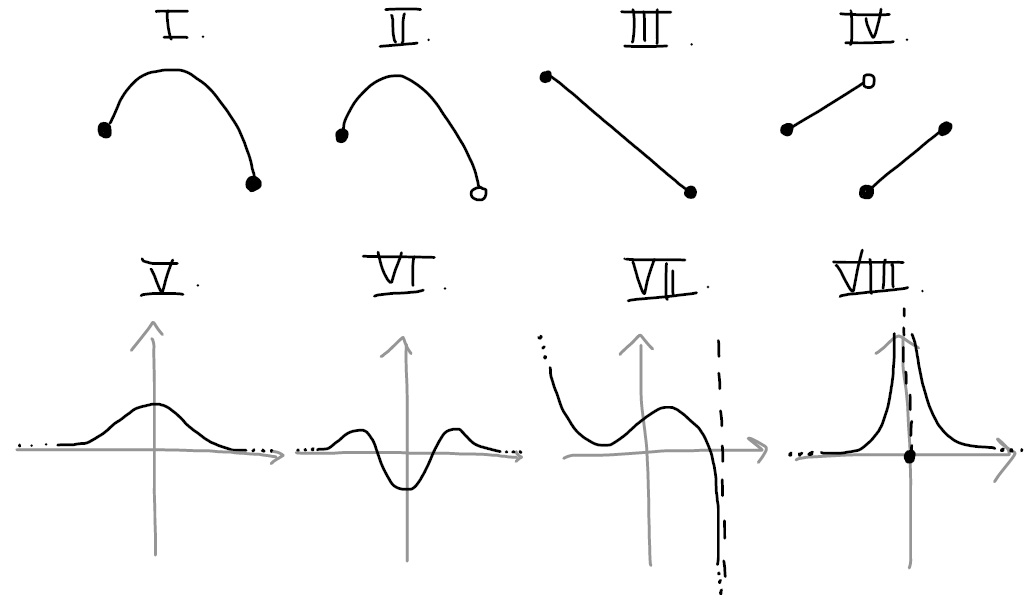
\includegraphics[width=7in]{graphs.jpg}
    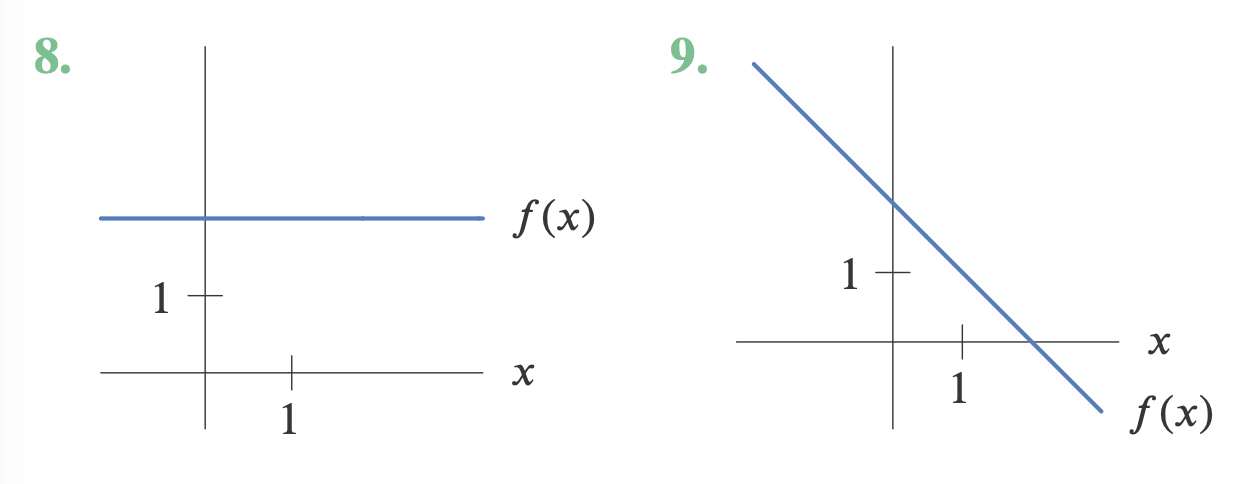
\includegraphics[width=3in]{Figures/graphs1}
    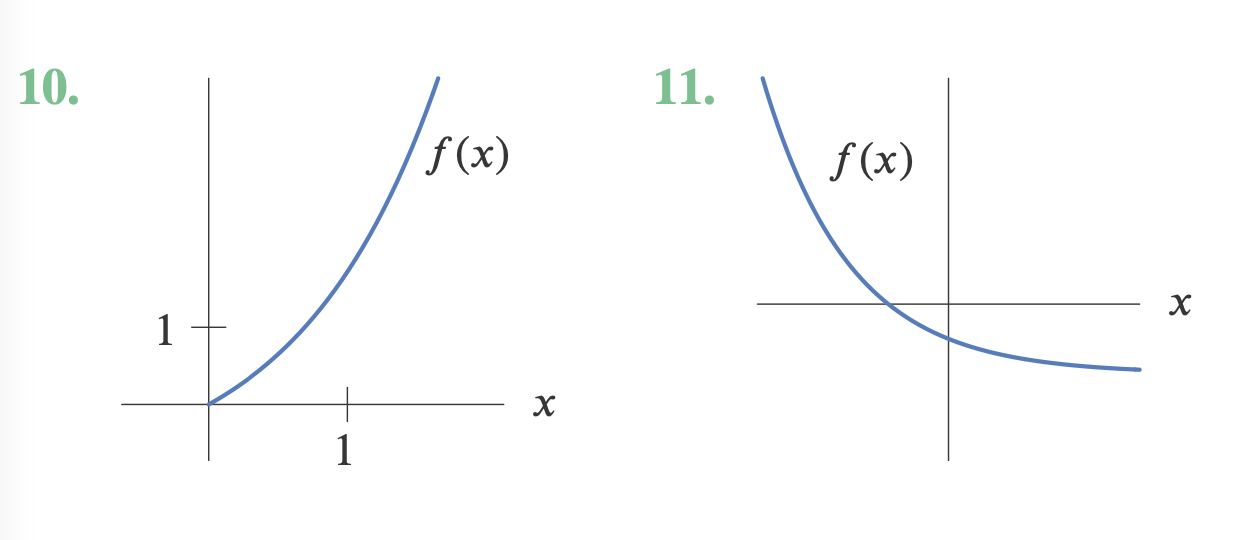
\includegraphics[width=3in]{Figures/graphs2}

    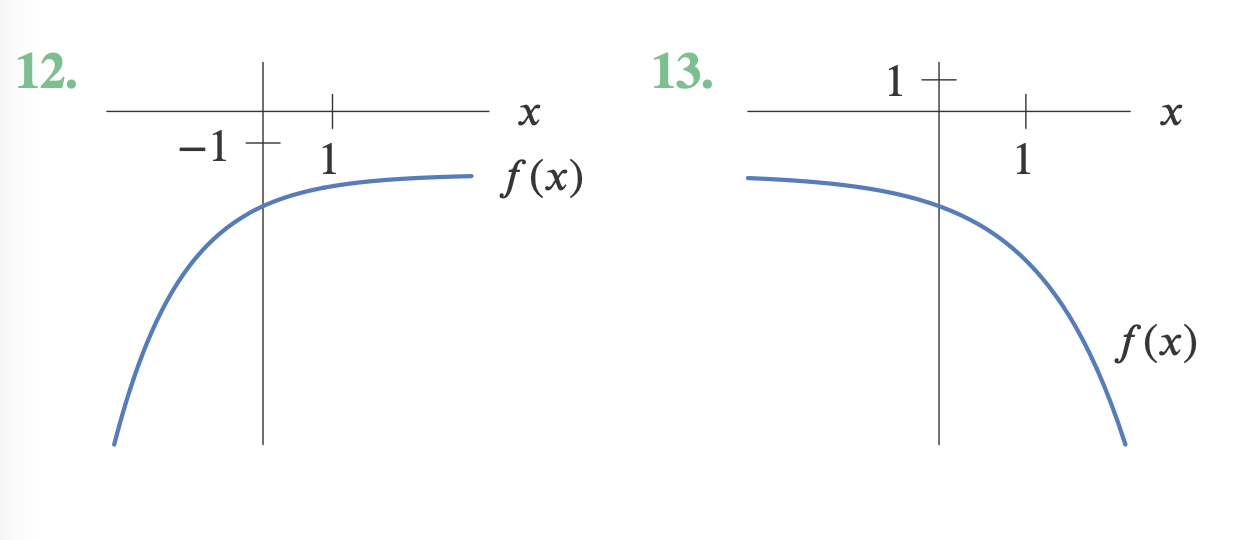
\includegraphics[width=3in]{Figures/graphs3}
\begin{solution}
  \begin{enumerate}
  \item[8.]  \(f'(x) = 0, f''(x) = 0\)
  \item[9.] \(f'(x)\) is negative, \(f''(x) = 0\)
  \item[10.] \(f'(x)\) is positive, \(f''(x)\) is positive
  \item[11.] \(f'(x)\) is negative, \(f''(x)\) is positive
  \item[12.] \(f'(x)\) is positive, \(f''(x)\) is negative
  \item[13.] \(f'(x)\) is negative, \(f''(x)\) is negative
  \end{enumerate}
\end{solution}
\question Define a position function $s(t)$ and suppose $s'(t)=v(t)$ is given in the following table.\\
\hspace*{.4cm}  What can you say about $v(t)$?  What about the acceleration function $v'(t)=a(t)$?

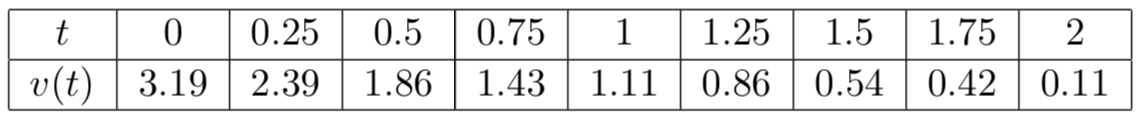
\includegraphics[width=4in]{Figures/table.jpg}
\begin{solution}
  \(v(t)\) appears to be increasing. However, \(a(t)\) appears to be
  positive and decreasing.
\end{solution}
\question At which of the marked \(x\)-values in the graph below can
  the following statements be true?\\
  \begin{minipage}{0.6\linewidth}
    \begin{enumerate}[(a)]
    \item \(f(x) < 0\)
    \item \(f'(x) < 0\)
    \item \(f(x)\) is decreasing
    \item \(f'(x)\) is decreasing
    \item The slope of the tangent lines of \(f(x)\) is positive
    \item The slope of the tangent lines of \(f(x)\) is increasing
    \end{enumerate}
  \end{minipage}
  \begin{minipage}{0.4\linewidth}
    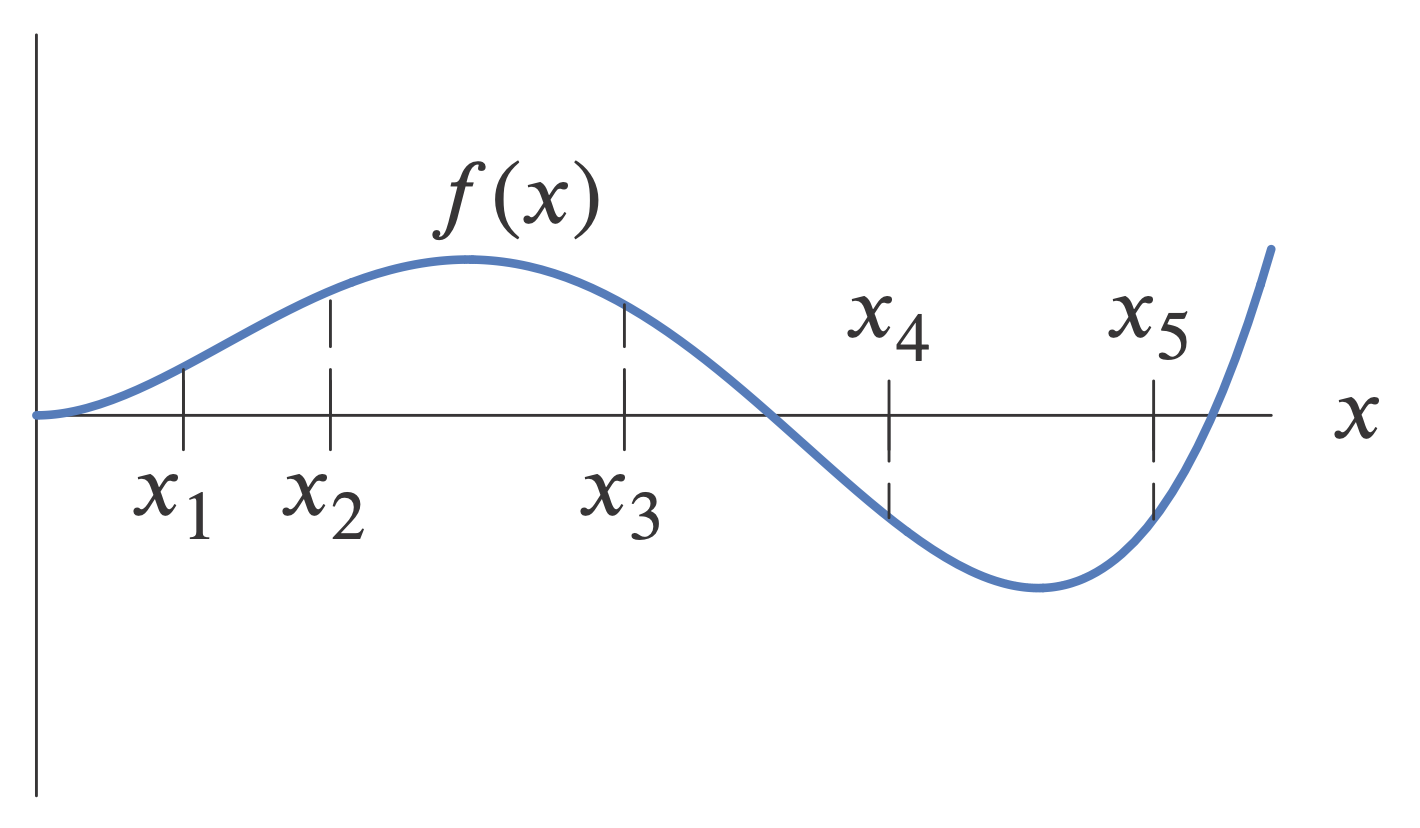
\includegraphics[width=2.5in]{Figures/figure256}
  \end{minipage}
  % 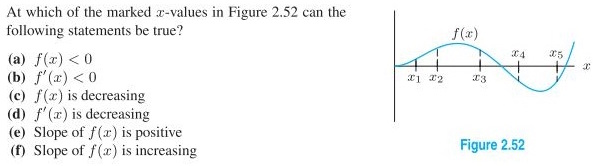
\includegraphics[width=7in]{no28.jpg}
  \begin{solution}
    \begin{enumerate}[(a)]
    \item \(x_4,x_5\)
    \item \(x_3,x_4\)
    \item \(x_3,x_4\)
    \item Possibly \(x_1\) (hard to tell) and definitely \(x_2,x_3\).
    \item \(x_1, x_2, x_5\)
    \item \(x_4, x_5\)
    \end{enumerate}
  \end{solution}
\question A function \(f\) has \(f(5) = 20, f'(5)=2\) and \(f''(x) <
  0\) for \(x \geq 5\). Which of the following are possible values for
  \(f(7)\) and which are impossible?
  \begin{center}
    (a) 26 \hspace{1.5in} (b) 24 \hspace{1.5in} (c) 22
  \end{center}
  \begin{solution}
    Since \(f'(5)\) is positive \(2\) and \(f''(x) < 0\) for \(x \geq
    5\), this means that the rate \(f\) is increasing by is
    decreasing. In other words, it must be that \(f(7) <
    f(5)+2*(7-5) = 24\). Therefore, (c) \(22\) is a possible answer,
    but (b) 24 and (a) 26 are impossible.
  \end{solution}
\question (Winter 2017 Exam 2) The graph of a portion of the derivative of $b(x)$ is shown below. Assume that $b(x)$ is defined and continuous on $[-5,6]$.
  \begin{center}
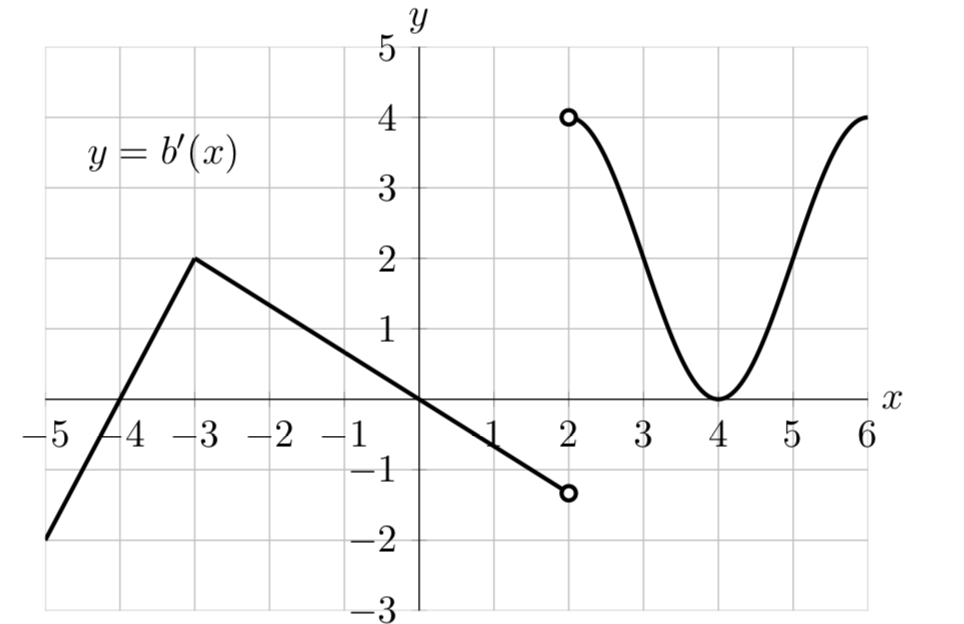
\includegraphics[scale=0.7]{Figures/graphb.png}
  \end{center}
For what values of $x$ is $b(x)$ concave up? Write your answer using inequalities or interval notation.
  \begin{solution}
    See \href{https://dhsp.math.lsa.umich.edu/exams/115exam2/w17/s1.pdf}{https://dhsp.math.lsa.umich.edu/exams/115exam2/w17/s1.pdf}
  \end{solution}

\question (Winter 2015 Exam 3) 	Shown on the axes below are the graphs of $y = f(x)$, $y = f'(x)$, and $y = f''(x)$. Determine which graph is which.
  \begin{center}
    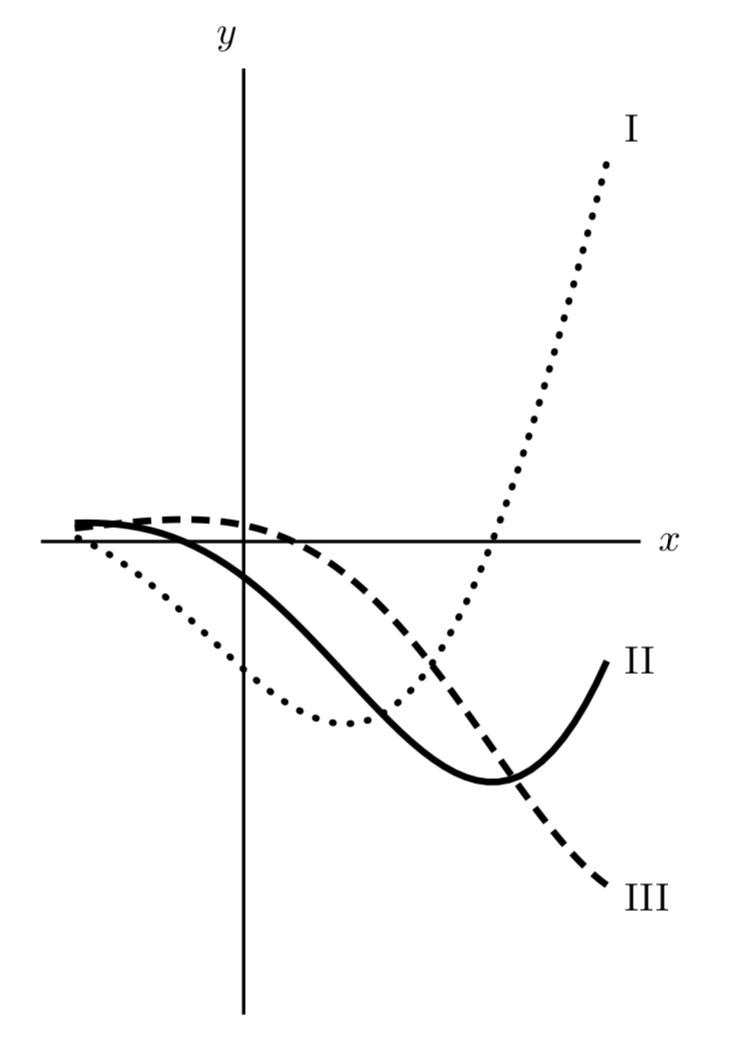
\includegraphics[scale=0.45]{Figures/match.png}
  \end{center}
  \begin{solution}
    \(f(x)\): III, \(f'(x)\): II, and \(f''(x)\): I\\
    Tricks for finding solution:
    \begin{enumerate}
    \item Look at where I, II, and III have tangent lines with slope
      \(0\). If their derivative is present, then there should be
      another function that crosses the \(x\)-axis at that
      point. Already, we can see I has no such corresponding function,
      so this tells us that it must be \(f''(x)\). Then, it crosses
      the \(x\)-axis where II has tangent lines of slope \(0\), so II
      must be \(f'(x)\) and similarly, this means III must be
      \(f(x)\).
    \item Look at where each function is increasing and decreasing, as
      well as where it is positive and negative. Then, you can match
      this information up using what we know about the relationship
      between derivatives and where functions are
      increasing/decreasing.
    \item Use concavity to figure out which function is \(f\) and
      which must be \(f''\). Then, double check your answer makes
      sense with one of the other methods above.
    \end{enumerate}
  \end{solution}
\question (Fall 2015 Exam 1) Below is the graph of $f^\prime(x)$, the \underline{\textbf{derivative}} of the function $f(x)$. Note that $f^\prime(x)$ is zero for $x \leqslant -2$, linear for $-2 < x < -1$, and constant for $-1 <x < 0$.
  \begin{center}
    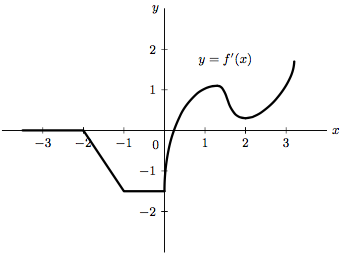
\includegraphics[scale=0.7]{Figures/graph_exam_problem.png}
  \end{center}
For each of the following, circle \underline{all} of the listed intervals for which the given statement is true over the entire interval. If there are no such intervals, circle NONE. You do not need to explain your reasoning.
\begin{enumerate}[(a)]
	\item $f^\prime(x)$ is increasing.
\[-2 < x < -1 \qquad 0 < x < 1 \qquad 1 < x < 2 \qquad 2 < x < 3 \qquad \text{NONE}\]
	\item $f^\prime(x)$ is concave up.
\[0<x<1 \qquad 1<x<2 \qquad 2<x<3 \qquad \text{NONE}\]
	\item $f(x)$ is increasing.
\[-2 < x < -1 \qquad -1 < x < 0 \qquad 0 < x < 1 \qquad 1 < x < 2 \qquad 2 < x < 3 \qquad \text{NONE}\]
	\item $f(x)$ is linear but not constant.
\[\hspace{-8ex}-3<x<-2 \qquad -2<x<-1 \qquad -1<x<0 \qquad 0<x<1 \qquad 1<x<2 \qquad 2<x<3 \qquad \text{NONE}\]
	\item $f(x)$ is constant.
\[\hspace{-8ex}-3<x<-2 \qquad -2<x<-1 \qquad -1<x<0 \qquad 0<x<1 \qquad 1<x<2 \qquad 2<x<3 \qquad \text{NONE}\]
\end{enumerate}
\begin{solution}
  See \href{https://dhsp.math.lsa.umich.edu/exams/115exam1/f15/s10.pdf}{https://dhsp.math.lsa.umich.edu/exams/115exam1/f15/s10.pdf}
\end{solution}
\question (Winter 2017 Exam 2) 	Some information about a function $f(x)$ is given in the table below.
	
$$\begin{array}{|c|c|c|c|c|c|c|c|}
\hline
	x &
-2 &
-1 &
0 &
1 &
2 &
3 &
4 \\
\hline
f'(x) &
-2 &
0 &
-2 &
0 &
1 &
0 &
-1 \\
\hline
f''(x) &
1 &
0 &
0 &
2 &
0 &
0 &
-2 \\
\hline
\end{array}$$
Assume that $f''(x)$ is continuous on $[-2,4]$ and that the values of $f'(x)$ and $f''(x)$ are strictly positive or strictly negative between consecutive table entries. Circle all of the intervals on which $f''(x)$ must be negative, if any exist.
$$-2 < x < -1 \quad -1 < x < 0 \quad 0 < x < 1 \quad 1 < x < 2
\quad 2<x<3 \quad 3<x<4 \quad \textrm{None of these}$$
\begin{solution}
  \(-1<x<0\), \(2<x<3\), \(3<x<4\). This follows since \(f'(x)\)
  is
  decreased on all those intervals and the problem states that
  \(f''(x)\) is strictly positive or strictly negative between
  consecutive table entries.
\end{solution}
\question (Winter 2016 Exam 1) 	The graph of a function $f$ is shown below.
  \begin{center}
    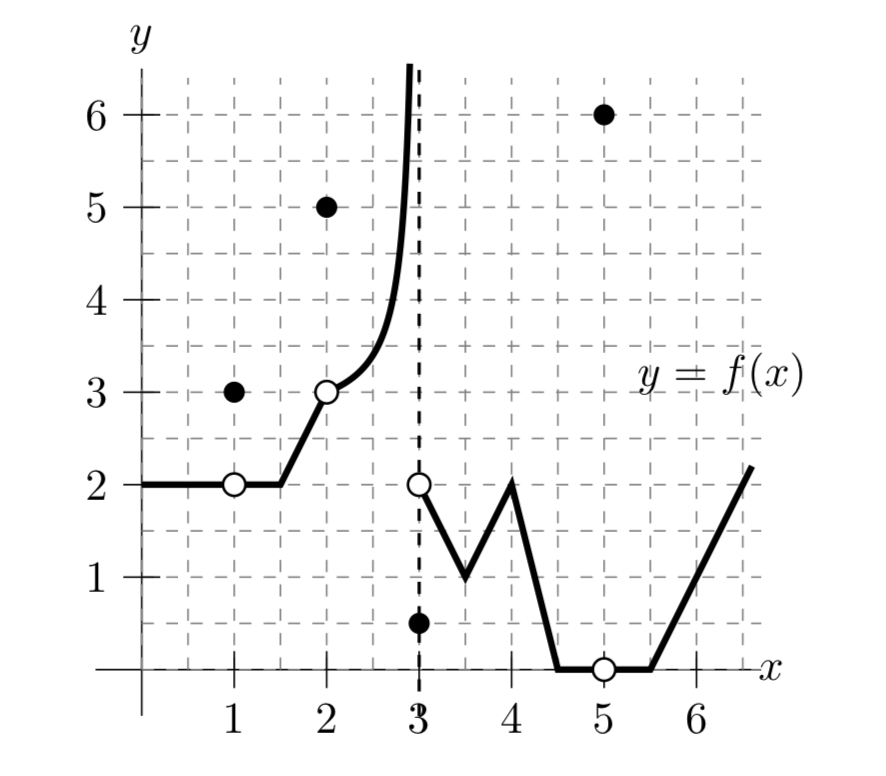
\includegraphics[scale=0.6]{Figures/discontinuities.png}
  \end{center}

Note: You may assume that pieces of the function that appear linear are indeed linear.
Use the graph above to evaluate each of the expressions below.
\begin{multicols}{2}
\begin{enumerate}[(a)]
	\item $f(1)$
	\item $\displaystyle\lim_{x \rightarrow 5} f(x)$
	\item $\displaystyle\lim_{q \rightarrow 3} f(q)$
	\item $\displaystyle\lim_{z \rightarrow 2} f(2)$
	\item $\displaystyle\lim_{r \rightarrow 6^-} f(r)$
	\item $\displaystyle\lim_{h \rightarrow 0} \frac{f(4.25+h)-f(4.25)}{h}$
	\item $\displaystyle\lim_{p \rightarrow 0.5} \frac{f(p)}{p}$
	\item $\displaystyle\lim_{t \rightarrow 3} f(t)f(t+2)$
	\item $\displaystyle\lim_{x \rightarrow 3^+} f(f(x))$
	\item $\displaystyle\lim_{s \rightarrow 1} f(f(s))$
\end{enumerate}
\end{multicols}
\begin{solution}
 See \href{https://dhsp.math.lsa.umich.edu/exams/115exam1/w16/s1.pdf}{https://dhsp.math.lsa.umich.edu/exams/115exam1/w16/s1.pdf}
\end{solution}
\end{questions}
\end{document}
%%% Local Variables:
%%% mode: latex
%%% TeX-master: t
%%% End:
